\documentclass[12pt]{article}
\font\tty=cmtt10 at 12truept
\title{A brief introduction to the \texttt{BOMdataRipper} package}
\author{Jason Lessels and Andrey Kostenko}


\usepackage{Sweave}
\begin{document}
\Sconcordance{concordance:BOMdataRipper-overview.tex:BOMdataRipper-overview.Rnw:%
1 6 1 1 0 9 1 1 2 1 0 1 1 3 0 1 2 2 1 1 2 4 0 1 2 2 1 1 2 1 0 1 1 3 0 2 %
2 1 0 2 1 1 2 1 0 2 1 3 0 1 2 1 1 2 2 4 1 1 2 1 0 2 1 3 0 1 4 2 0 1 2 1 %
0 1 4 6 0 1 2 1 4 1 2 7 1 1 4 3 0 1 1 1 2 1 0 1 4 6 0 1 3 1 0 4 1 1 3 5 %
0 3 2 1 1 1 4 3 0 1 1 1 2 1 0 1 1 3 0 1 10 8 0 6 1 3 0 1 3 1 0 1 2 1 0 %
6 1 1 2 1 1 1 2 1 0 1 1 1 3 2 0 1 2 1 0 5 1 3 0 1 6 4 0 1 1 1 4 6 0 1 4 %
1 2 4 1}


\maketitle

\section{Introduction}
This is intended to provide a brief overview of the functionality of the package.

Load the package and the database with all sites: 

\begin{Schunk}
\begin{Sinput}
> library(BOMdataRipper)
> all_sites <- allBOMSites()
\end{Sinput}
\end{Schunk}

By default the \texttt{allBOMSites} fucntion examines the database and updates the database if it is 30 days or older. However, if the user would like to update the database manually this can be achieved using:

\begin{Schunk}
\begin{Sinput}
> all_sites <- allBOMSites(force_db_update = TRUE)
\end{Sinput}
\end{Schunk}

\section{Plot the location of all active sites across Australia}
The \texttt{allBOMSites} function returns a data.frame with statistics and the geographical location of each station. All sites can be subsetted to remove all non-active sites. 
\begin{Schunk}
\begin{Sinput}
> active_sites_index <- all_sites$stillActive=="Y"
> active_sites <-  subset(all_sites, active_sites_index)
\end{Sinput}
\end{Schunk}
Using the \texttt{ggmap} package a simple map showing the location of all the points can be created. 
\begin{Schunk}
\begin{Sinput}
> require(ggmap)
> australia = get_map(location = "Australia", zoom=4)
> australia_map = ggmap(australia)
> # Subset the active sites for plotting
> active_sites_index <- all_sites$stillActive=="Y"
> active_sites <-  subset(all_sites, active_sites_index)
> australia_map + geom_point(aes(long,lat), data=active_sites)
\end{Sinput}
\end{Schunk}
\begin{center}
\begin{figure}
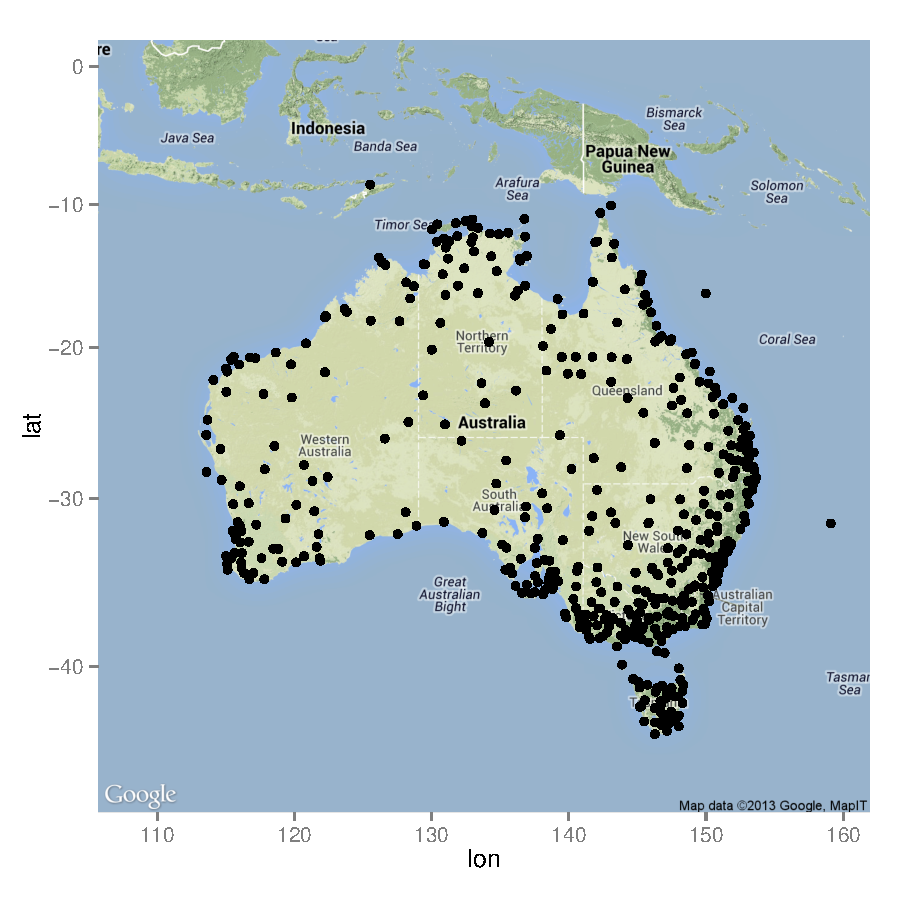
\includegraphics{BOMdataRipper-overview-005}
\caption{Location of meterological sites across Australia}
\end{figure}
\end{center}
\section{Downloading daily rainfall data in Sydney}

\begin{Schunk}
\begin{Sinput}
> site_index <- str_detect(tolower(all_sites$stationName), "penrith lakes")
> penrith_station_number <- all_sites[site_index, "stationNumber"]
> rainfall <- bomDailyObs(penrith_station_number, observation="rain")
\end{Sinput}
\end{Schunk}
\begin{Schunk}
\begin{Sinput}
> # load the ggthemes package to help with plotting
> library(ggthemes)
> # Add a new column with zeros for plottiing
> rainfall$zeros <- rep(0, nrow(rainfall))
> # plot it using geom_segments
> ggplot() + geom_segment(aes(y=rainfall,yend=zeros, x=date, xend=date), 
+                         rainfall) + theme_few() + 
+   xlab("date") + ylab("rainfall (mm)")
\end{Sinput}
\end{Schunk}
\begin{figure}
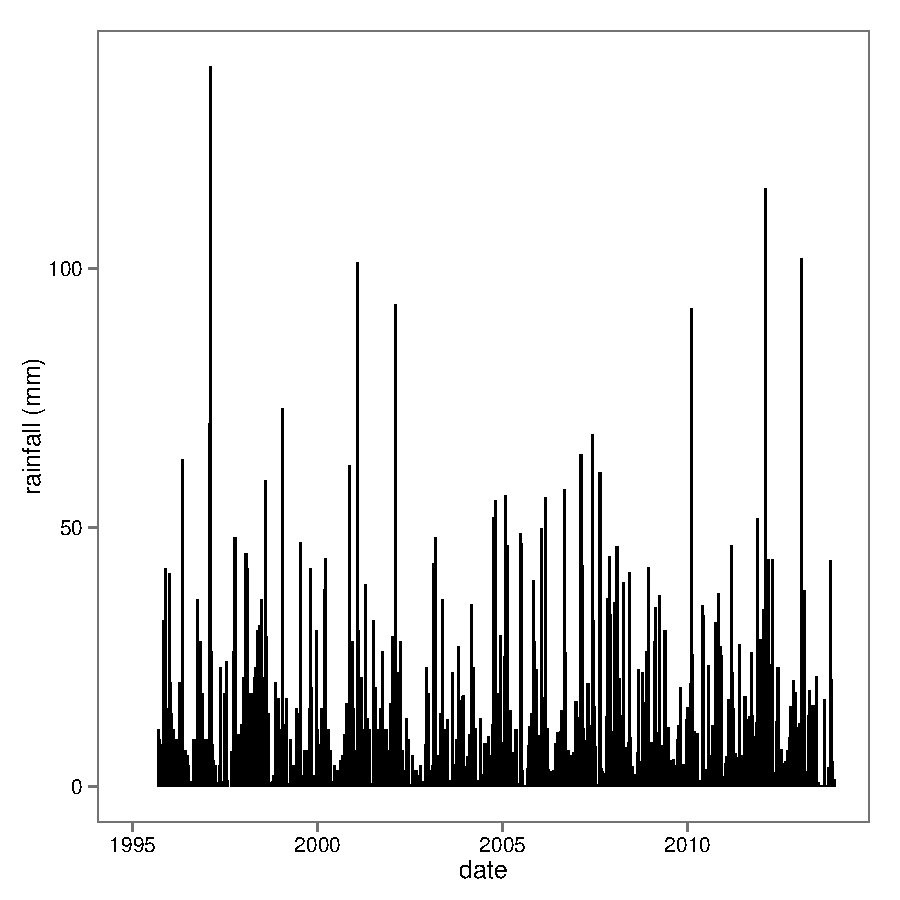
\includegraphics{BOMdataRipper-overview-008}
\caption{Daily rainfall data for Penrith Lakes, NSW}
\end{figure}

\newpage

\section{Downloading and mapping monthly rainfall in Sydney}
This section outlines how metrological sites within a certain area can be found and the data for these sites can be easily downloaded. A brief example of spatcetime prediction of monthly rainfall data is also provided. 

\begin{Schunk}
\begin{Sinput}
> #Get the statilite image from google.
> sydney = get_map(location = "Blacktown, NSW, Australia",
+                  zoom=10, maptype = 'satellite')
> sydney_map = ggmap(sydney)
> # Get the extent of the plot.
> bounding_box <- sydney_map[[1]]
> sydney_site_index <- all_sites$lat>bounding_box$lat[1]&
+   all_sites$long>bounding_box$lon[1]&
+   all_sites$long<bounding_box$lon[4]&
+   all_sites$lat<bounding_box$lat[4]
\end{Sinput}
\end{Schunk}
\begin{Schunk}
\begin{Sinput}
> sydney_rainfall_sites <- all_sites[sydney_site_index, ]
> syndey_active_sites <- sydney_rainfall_sites$stillActive =="Y"
> sydney_rainfall_sites <- sydney_rainfall_sites[syndey_active_sites,]
> remove_nas <- !is.na(sydney_rainfall_sites$stationNumber)
> sydney_rainfall_sites <- subset(sydney_rainfall_sites, remove_nas)
> sydney_map + 
+   geom_point(aes(x=long, y=lat),col="red", size=10, 
+              data=sydney_rainfall_sites)
\end{Sinput}
\end{Schunk}
\begin{figure}
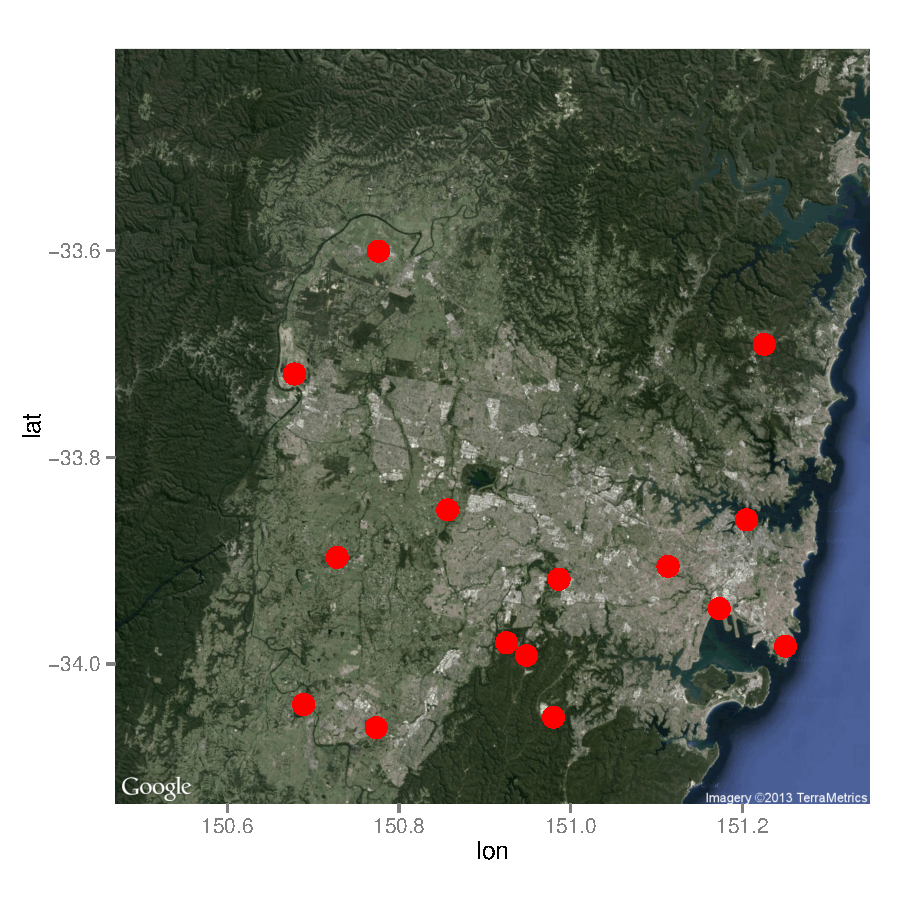
\includegraphics{BOMdataRipper-overview-011}
\caption{Map of Sydney area with active meterological stations.}
\end{figure}
\begin{Schunk}
\begin{Sinput}
> ## Download the monthly rainfall of each site. 
> annualRain <- lapply(1:nrow(sydney_rainfall_sites), function(i) 
+   try(bomMonthlyObs(sydney_rainfall_sites$stationNumber[i],"rain")))
> names(annualRain) <- sydney_rainfall_sites$stationNumber
> ### Format the downloaded data
> fail_index <- sapply(annualRain, function(x) !inherits(x, "try-error"))
> annualRain <- annualRain[fail_index]
\end{Sinput}
\end{Schunk}
\begin{Schunk}
\begin{Sinput}
> get2012 <- function(x){
+   index <- x$year==2012
+   if(sum(index)>0){
+     x$observation[index]
+   } else {
+     NA
+   }
+ }
> rain_2012<- lapply(1:length(annualRain),function(i) get2012(annualRain[[i]][[1]]))
> names(rain_2012) <- names(annualRain)
> no_data <-sapply(rain_2012, function(x) !any(is.na(x)))
> rain_2012 <- rain_2012[no_data]
> merged_data <- do.call("cbind",rain_2012)
> rain_data = data.frame(date = as.Date(ymd(paste(2012, 1:12, 1))), merged_data)
\end{Sinput}
\end{Schunk}
\begin{Schunk}
\begin{Sinput}
> library(gstat)
> coor_index <- match(str_replace(names(rain_data[-1]), "X", ""), 
+                     sydney_rainfall_sites$stationNumber)
> syd_rain <- sydney_rainfall_sites[coor_index,]
> syd_rain$y <- syd_rain$lat
> syd_rain$x <- syd_rain$long
> coordinates(syd_rain)<- ~x+y
> proj4string(syd_rain) = "+proj=longlat +datum=WGS84"
> plot(syd_rain)
> pts <- coordinates(syd_rain)
> rownames(pts) <- syd_rain$stationNumber
> pts = SpatialPoints(pts, 
+                     CRS("+proj=longlat +datum=WGS84 +ellps=WGS84 +towgs84=0,0,0"))
> library(spacetime)
> rain.data = stConstruct(rain_data[,-1], 
+                         space = list(values = 1:ncol(rain_data[,-1])),
+                         time = rain_data[,1], SpatialObj = pts, interval = TRUE)
> grid <- SpatialPixels(SpatialPoints(makegrid(pts, n=1000)), 
+                       proj4string= "+proj=longlat +datum=WGS84 +ellps=WGS84 +towgs84=0,0,0")
> library(xts)
> tgrd = rain_data[,1]
> pred.grid = STF(grid, tgrd)
> v = vgmST("separable", space = vgm(1, "Exp", 75), time = vgm(1, "Exp", 1.5), sill=0.6)
> rain.ST = krigeST(values ~ 1, rain.data, pred.grid, v)
\end{Sinput}
\end{Schunk}
\begin{Schunk}
\begin{Sinput}
> predicted = data.frame(coordinates(rain.ST), 
+                        time = rep(rain_data[,1], each= length(grid)),
+                        pred = rain.ST@data, 
+                        fdate = as.factor(rep(rain_data[,1], each=length(grid))))
> names(predicted) = c("x", "y", "date", "rain", "fdate")
> ggplot() + 
+   geom_raster(aes(x, y, fill=rain), predicted, alpha=0.5) +
+   facet_wrap(~fdate) +
+   scale_fill_gradient(low = "steelblue",high = "red") 
\end{Sinput}
\end{Schunk}
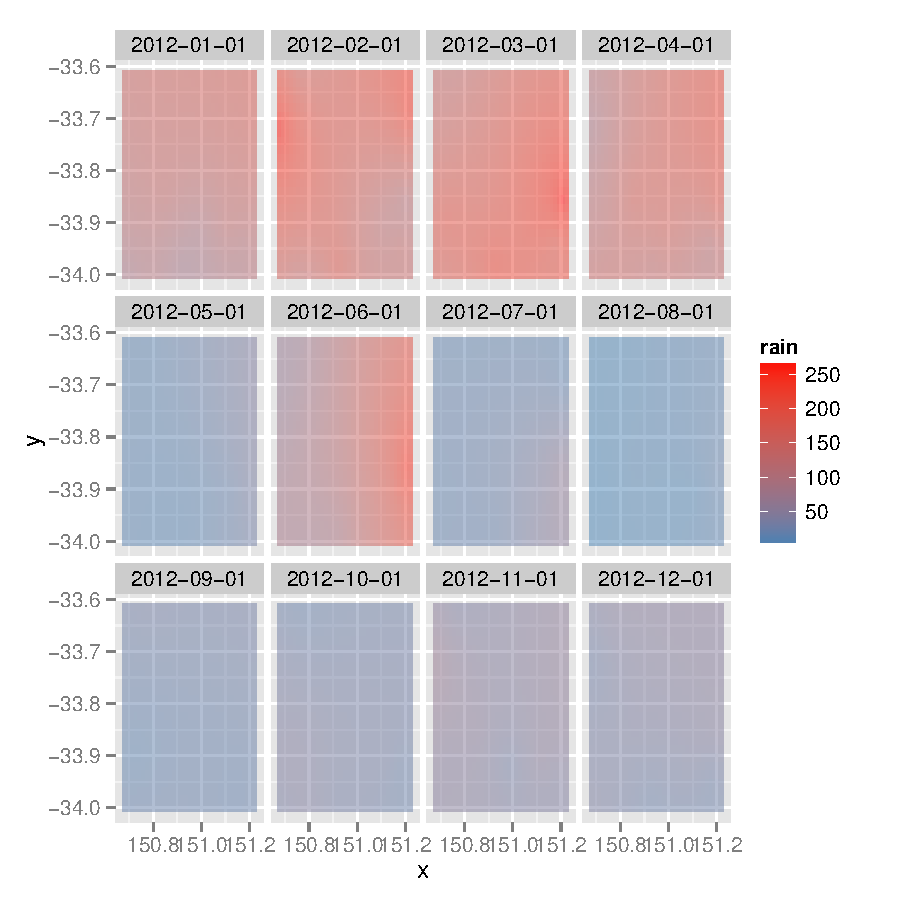
\includegraphics{BOMdataRipper-overview-016}




\end{document}
